\documentclass[12pt,spanish,fleqn,openany,letterpaper,pagesize]{scrbook}

\usepackage[utf8]{inputenc}
\usepackage[spanish]{babel}
\usepackage{fancyhdr}
\usepackage{epsfig}
\usepackage{epic}
\usepackage{eepic}
\usepackage{amsmath}
\usepackage{threeparttable}
\usepackage{amscd}
\usepackage{here}
\usepackage{graphicx}
\usepackage{lscape}
\usepackage{tabularx}
\usepackage{subfigure}
\usepackage{longtable}


\usepackage{rotating} %Para rotar texto, objetos y tablas seite. No se ve en DVI solo en PS. Seite 328 Hundebuch
                        %se usa junto con \rotate, \sidewidestable ....


\renewcommand{\theequation}{\thechapter-\arabic{equation}}
\renewcommand{\thefigure}{\textbf{\thechapter-\arabic{figure}}}
\renewcommand{\thetable}{\textbf{\thechapter-\arabic{table}}}


\pagestyle{fancyplain}%\addtolength{\headwidth}{\marginparwidth}
\textheight22.5cm \topmargin0cm \textwidth16.5cm
\oddsidemargin0.5cm \evensidemargin-0.5cm%
\renewcommand{\chaptermark}[1]{\markboth{\thechapter\; #1}{}}
\renewcommand{\sectionmark}[1]{\markright{\thesection\; #1}}
\lhead[\fancyplain{}{\thepage}]{\fancyplain{}{\rightmark}}
\rhead[\fancyplain{}{\leftmark}]{\fancyplain{}{\thepage}}
\fancyfoot{}
\thispagestyle{fancy}%


\addtolength{\headwidth}{0cm}
\unitlength1mm %Define la unidad LE para Figuras
\mathindent0cm %Define la distancia de las formulas al texto,  fleqn las descentra
\marginparwidth0cm
\parindent0cm %Define la distancia de la primera linea de un parrafo a la margen

%Para tablas,  redefine el backschlash en tablas donde se define la posici\'{o}n del texto en las
%casillas (con \centering \raggedright o \raggedleft)
\newcommand{\PreserveBackslash}[1]{\let\temp=\\#1\let\\=\temp}
\let\PBS=\PreserveBackslash

%Espacio entre lineas
\renewcommand{\baselinestretch}{1.1}

%Neuer Befehl f\"{u}r die Tabelle Eigenschaften der Aktivkohlen
\newcommand{\arr}[1]{\raisebox{1.5ex}[0cm][0cm]{#1}}

%Neue Kommandos
\usepackage{Befehle}


%Trennungsliste
\hyphenation {Reaktor-ab-me-ssun-gen Gas-zu-sa-mmen-set-zung
Raum-gesch-win-dig-keit Durch-fluss Stick-stoff-gemisch
Ad-sorp-tions-tem-pe-ra-tur Klein-schmidt
Kohlen-stoff-Mole-kular-siebe Py-rolysat-aus-beu-te
Trans-port-vor-gan-ge}

\begin{document}

\justifying

\section{Machine Learning}

  \par Existen numerosos autores que han definido el concepto de que una máquina
    aprende, en este trabajo hemos extraído una en particular que resulta
    clara
    \begin{framed}
      \begin{center}
        \textit{Se dice que un programa de computadora \textbf{aprende} de experiencia
        $E$ con respecto a alguna tarea $T$ y una métrica de rendimiento $M$, si
        con la experiencia $E$ se incrementa su rendimiento en la tarea $T$,
        medida por $M$.}\\
      \end{center}
      \centering \textbf{Tom Mitchell, 1997} \cite{mitchell_learn}
    \end{framed}

    También, en el mismo libro, Mitchell enuncia que el campo del aprendizaje
    automático se refiere a la cuestión de cómo construir programas
    que mejoren automáticamente con experiencia.
    En ese marco, luego de muchos avances en el área, podemos decir que el
    \textit{Aprendizaje Automático} (ML) es un
    enfoque empírico efectivo para regresiones y/o clasificaciones de sistemas
    lineales y no lineales, que pueden involucrar desde unos pocos hasta varios
    cientos de variables.

  \par Además, los métodos de ML se pueden clasificar en
    \textit{supervisados}\cite{supervised_learning} y
    \textit{no-supervisados}\cite{unsupervised_learning}, aunque hoy en día
    existen matices entre estas dos clases\cite{semi_supervised}.
    Los algoritmos que aprenden a través de métodos supervisados son aquellos que
    aprenden una función que mapea un valor de entrada a uno de salida basado
    en pares de ejemplos entrada-salida.
    El caso de los algoritmos que utilizan métodos no-supervisados aprenden
    realizando inferencia de la función que describe la estructura de los datos
    de ejemplo. En este caso, los datos de entrenamiento del algoritmo no son
    etiquetados (no existen pares entrada-salida de ejemplo).

  \par Los algoritmos bajo el enfoque de ML requieren entrenamiento utilizando un
    conjunto de datos que sea representativo del conjunto del problema.
    Además, para lograr modelos que puedan generalizar a datos nunca antes vistos,
    los algoritmos supervisados necesitan dos subconjuntos necesariamente
    disjuntos de datos: el conjunto de entrenamiento y el de validación\cite{test_val}


  \par El ML es ideal para aquellos problemas en donde el conocimiento teórico del mismo
    es incompleto o insuficiente, pero se cuenta con un gran conjunto de observaciones.
    Este enfoque se utiliza, de manera creciente a medida que pasa el tiempo y
    el poder de cómputo se incrementa, en gran cantidad de aplicaciones tanto para
    problemas más relacionados al ámbito científico, como para problemas
    industriales. Algunos ejemplos de lo primero van desde problemas de
    procesamiento de lenguaje
    natural\cite{twitt_nlp, cardellino, svm_semantic}, procesamiento de
    imágenes\cite{face_detection, corner_detection, handwritting} hasta aplicaciones
    en el área de la salud\cite{nutrition_prediction, bigdata_health, age_estimation, children}
    y las Geociencias\cite{solar_irradiation, ml_grs, modeling_mineral}.

  \par Estas técnicas han mostrado ser de utilidad para un gran número de
    aplicaciones en Geociencias relacionadas a la tierra, oceanos y atmósfera,
    y en algoritmos de extracción de información bio-geofísica.
    Algunos de los algoritmos de ML más usados en aplicaciones relativas a
    Geociencias y Sensado Remoto (GRS) son las Redes Neuronales Artificiales (ANN),
    Support Vector Machines (SVM), Mapas Auto-organizados (SOM), Árboles de Decisión (DT),
    Random Forests y Algoritmos Genéticos. Su aplicación en problemas de GRS es
    relativamente nuevo y extremádamente prometedor. En particular, ANNs son
    usadas para clasificación y la aplicación en pronósticos
    relativos a series de tiempo.

  \par Una exploración en la base bibliográfica \textit{Scopus} (\url{www.scopus.com})
    devuelve más de 2.000 publicaciones que incluyen \textit{remote sensing} y
    \textit{machine learning} donde unas 900 fueron publicadas hasta el 2015, y
    alrededor de 1.200 desde ese año hasta la actualidad. Del total, el 24.5\% se
    corresponde con el área de \textit{Computer Science}, un 21.3\% a
    \textit{Earth and Planetary Sciences}, 16.5\% a \textit{Engineering} y el
    restante 37.7\% se distribuye entre numerosas áreas. Esta búsqueda reflejó
    que China, Estados Unidos, Alemania e Italia son los países con mayor
    producción en este sentido.

  \par A su vez, para tener una noción más exhaustiva sobre los esfuerzos académicos
    al respecto de los tópicos que se tratan en este trabajo, se realizó un búsqueda
    sobre la relación entre algunas de la herramientas que se han utilizado y
    el \textit{remote sensing}.

  \par Se encontró que si se cambian las palabras clave por
    \textit{remote sensing} y \textit{neural network} \textit{Scopus} muestra
    que existen 4.000 publicaciones con esos tópicos, de las cuales alrededor de
    1.500 fueron desde el 2015 hasta la actualidad. Del total, un 23.8\% se
    corresponde con el área de \textit{Computer Science}, un 22.7\% a
    \textit{Earth and Planetary Sciences}, 17.5\% a \textit{Engineering} y el
    restante 36\% se distribuye otras áreas; con China,
    Estados Unidos, Italia e India como los paises con mayor producción
    científica en dichas áreas.
    El hecho de que esta búsqueda haya arrojado más resultados que la mencionada
    anteriormente, indica que es posible que los investigadores que estén trabajando
    sobre problemáticas de este tipo, quizás, no están explotando las grandes
    capacidades del área de aprendizaje automático en su extensión y, en vez de
    eso, se están centrando en utilizar ANNs por su alta popularidad.

  \par Otra exploración, esta vez sobre \textit{remote sensing} y \textit{k nearest},
    arroja unos 1.100 resultados, de los cuales 310 fueron publicados desde
    el año 2015 a la actualidad. Esta vez, del total de publicaciones encontradas,
    un 25.7\% se corresponde con \textit{Earth and Planetary Sciences}, 16.1\%
    a \textit{Computer Science} y 15\% a \textit{Engineering}. Para este caso,
    Estados Unidos lidera fuertemente la lista de paises con más producción,
    con 387 trabajos. China y Alemania lo siguen con 320 publicaciones entre
    los dos.


  \par A continuación, expondremos de manera más detallada
    herramientas y métodos que motivaron el desarrollo del presente
    trabajo. Enfocaremos en los métodos de regresión, dado que es ésta la clase
    de problema que abordaremos. A su vez, los algoritmos que describiremos son
    los implementados por la librería \textit{Scikit-learn}.

\subsection{Scikit-learn}

  \par \textit{Scikit-learn}\cite{scikit-learn, sklearn_review} es una librería
    de Python de libre acceso para Aprendizaje Automático
    construido sobre \textit{SciPy}\cite{scipy}. Es una herramienta
    sencilla y efectiva para minería de datos y análisis de datos. Dado que está bajo
    licencia \textit{BSD}, esta librería puede ser utilizada tanto
    para uso personal como comercial.

  \par Este proyecto inició en el 2007 como un proyecto del \textit{Google Summer Scool} por David
    Cournapeau. Más tarde ese año, Matthieu Brucher comenzó a trabajar en éste proyecto
    como parte de su tesis. En 2010 Fabian Pedrafosa, Gael Varoquaux, Alexandre
    Gramfort y Vincent Michel del INRIA \footnote{Institut National de Recherche
    en Informatique et en Automatique} tomaron el liderazgo del proyecto y lo liberaron
    al público por primera vez, el 1ro de Febrero de 2010. Desde entonces, salieron muchos
    \textit{releases} siguiendo ciclos de 3 meses, y una gran comunidad internacional
    ha estado liderando el desarrollo desde entonces.

  \par Con scikit-learn, los usuarios pueden realizar una gran variedad de tareas
    que van desde selección de modelos, clustering, y preprocesamiento de datos, entre otras.
    La librería provee un completo conjunto de tareas que permiten una
    implementación completa de la solución de un problema de ML.

  \par Por las razones mencionadas es que tiene una muy extensiva utilización.
    Se está utilizando tanto para uso científico como en
    grandes compañias de diferentes industrias desde streaming de música, hasta
    recomendadores de hoteles, entre otras. Esto da la pauta de que los usuarios pueden
    integrar algoritmos implementados con este módulo a sus propias aplicaciones.

  \par Otra de las grandes bondades de la herramienta es que se asegura que
    tanto usuarios experimentados como aquellos que son nuevos puedan obtener
    la asistencia que necesitan para integrar el módulo de ML a sus propias
    plataformas, por ello es el alto nivel de detalle en su documentación oficial.



\subsection{Métodos Lineales}

  \par En este trabajo utilizamos dos tipos de regresiones lineales. La regresión
  lineal ordinaria, correspondiente al método de \textit{Mínimos Cuadrados}\cite{least_square}
  y método de regresión \textit{Ridge}\cite{ridge}.
  Dada su popularidad y simplicidad, no ahondaremos en explicaciones profundas
  con el fin de evitar detalles tediosos, muy conocidos.


\subsection{Árboles de Decisión}
  \par Los \textit{Árboles de Decisión} (DTs)\cite{decision_tree_regression}
    son métodos no paramétricos de aprendizaje supervisado
    utilizados tanto para problemas de clasificación como de regresión.
    La meta es crear un modelo que prediga el valor de una variable objetivo aprendiendo
    simples reglas de decisión inferidas a partir de las características de los datos
    de entrenamiento.


  \par El algoritmo de los DT construye modelos de clasificación o regresión
    utilizando una estructura arbórea. Éste divide el conjunto de datos en pequeños
    subconjuntos mientras que, al mismo tiempo, un árbol de decisión es incrementalmente
    construido. El resultado final es un árbol con nodos de decisión y nodos hojas.
    Un nodo de decisión tiene dos o más ramas, cada una representando valores para
    el atributo examinado. Un nodo hoja representa una decisión dentro del
    objetivo numérico. Los árboles de decisión pueden manejar tanto datos
    categóricos como numéricos.


  \par Más formalmente, dados los vectores de entrenamiento $x_{i} \in \mathbb{R}^{n}$, $i = 1,..,l$
    y un vector de etiquetas $y \in \mathbb{R}^{l}$, un árbol de decisión particiona
    recursivamente el espacio de modo que las muestras con la misma etiqueta se agrupen juntas.


  \par Supongamos que los datos en el nodo $m$ son representados por $Q$. Para cada
    candidato se divide $\theta = (j, t_{m})$ donde $j$ es una característica y
    $t_{m}$ es un humbral, particionando los datos en conjuntos $Q_{izq}(\theta)$ y
    $Q_{der}(\theta)$ donde:
    \begin{align}
      Q_{izq}(\theta) &= (x, y) | x_{j} \leq t_m \\
      Q_{der}(\theta) &= Q - Q_{izq}(\theta)
    \end{align}
    La impureza en $m$ es calculada usando la función de impureza $H()$, la elección
    de ésta depende de la tarea que se quiera realizar.
    En el caso de una regresión, para el nodo $m$, representando una
    región $R_{m}$ con una cantidad $N_{m}$ observaciones, los criterios
    para minimizar en cuanto a la determinación de ubicaciones para divisiones
    futuras suelen ser el \textbf{Error Cuadrático Medio}, que minimiza el error $L2$ usando
    valores promedios en los nodos terminales, y el \textbf{Error Absoluto Medio}, que minimiza
    el error $L1$ usando el valor de la mediana estadística en los nodos terminales.
    Luego, la función de impureza es
    \begin{align}
      G(Q, \theta) = \frac{n_{izq}}{N_{m}} \ H(Q_{izq}(\theta)) + \frac{n_{der}}{N_{m}} \ H(Q_{der}(\theta))
    \end{align}
    y se seleccionan los parámetros que minimicen la impureza tal como expresa la
    siguiente ecuación
    \begin{align}
      \theta^{*} = argmin_{\theta} \ G(Q, \theta)
    \end{align}

    Luego se sigue partiendo $Q_{izq}$ y $Q_{der}$ hasta que se alcance la profundidad
    máxima permitida del árbol, $N_{m} < min_{muestras}$ o bien $N_{m} = 1$


\subsection{Random Forest}

  \par \textit{Random Forest} (RF) es un método de aprendizaje que utiliza ensamblado y se
    usa para llevar a cabo tareas tanto de clasificación como de regresión.
    La idea es construir una variedad de árboles de decisión en tiempo de entrenamiento
    y devolver la clase que se corresponda con la moda estadística de las clases
    (para clasificación) o bien el promedio (para regresión) de los resultados
    obtenidos por los árboles individuales.

  \par Existen varios algoritmos de RF, describiremos formalmente el desarrollado
    por Breiman \cite{random_forest}.
    Sea $\mathcal{D}_{n} = \ \{ (X_{1}, Y_{1}), \ \dots, \ (X_{n}, Y_{n})\}$
    un conjunto de variables aleatorias independientes e idénticamente distribuídas (i.i.d.)
    pertenecientes al conjunto $[0,1]^{d} \ \times \ \mathbb{R} $ con $d \geq 2$,
    con la misma distribución que un par genérico $(X,Y)$ satisfaciendo que
    $\mathbbm{E}Y^{2} < \infty$. Además, sea $r()$ la función de regresión que se busca estimar.

  \par Un RF es un predictor que consiste de una colección aleatoria base
    de árboles de regresión, $\{ r_{n}(x, \theta_{m}, \mathcal{D}_{n}), m \ > \ 1 \}$, donde
    $\theta_{1},\ \theta_{2},\ \dots$ son salidas i.i.d. de una variable aleatoria
    $\theta$. Éstos árboles aleatorios son combinados para formar la estimación
    de la regresión:

    \begin{align}
      \overline{r}(X,\ \mathcal{D}_{n})\ =\ \mathbbm{E}_{\theta}[r_{n}(X,\ \theta,\ \mathcal{D}_{n})]
    \end{align}

    donde $\mathbbm{E}_{\theta}$ denota la esperanza con respecto al parámetro aleatorio
    condicionada por $X$ y el conjunto de datos $\mathcal{D}_{n}$. Notemos que
    dicha esperanza es evualuada por el método de Monte Carlo\cite{monte_carlo},
    esto es, generando $M$ árboles aleatorios, y tomando el promedio de los resultados.
    La variable de aleatoriedad $\theta$ es usada para determinar cómo se van a realizar los
    sucesivos cortes cuando se construyen los árboles individuales, como una selección
    de la coordenada a dividir y la posición de la división.

  \par Cada árbol aleatorio es construido de la siguiente manera: todos los nodos
    del árbol son asociados a celdas rectangulares tales que en cada etapa de
    construcción del árbol, el conjunto de celdas asociadas a las hojas del árbol
    forman una partición de $[0, 1]^{d}$. La raíz del árbol es exactamente $[0, 1]^{d}$.
    Luego, el siguiente procedimiento es repetido una cantidad $\lceil \log_{2}k_{n} \rceil$ veces
    donde $k_{n}$ es un parámetro determinístico, fijado por el usuario, posiblemente
    dependiente del valor de $n$.

    \begin{enumerate}
      \item En cada nodo, se selecciona una coordenada de $X = (X^{(1)}, \ \dots,\ X^{(d)})$
            donde la característica j-ésima tiene una probabilidad de $p_{nj} \in (0,1)$
            de ser elegida.
      \item En cada nodo, una vez que la coordenada es seleccionada, la división es
            en el punto intermedio del lado elegido.
    \end{enumerate}

    Cada árbol aleatorio $r_{n}(X, \theta)$ devuelve el promedio sobre todos los
    $Y_{i}$ para los cuales los vectores correspondientes $X_{i}$ caen en la misma
    celda de la partición aleatoria que $X$.


\subsection{K-Vecinos más cercanos (KNN)}
  \par El principio detrás de los métodos de vecinos más cercanos es encontrar un
    número predefinido de las muestras de entrenamiento más cercanas en distancia
    al nuevo punto, y predecir su valor a partir de ellos.
    El número de muestras puede ser una constante definida por el usuario, o
    variar basada en la densidad local de los puntos. La distancia puede, en general,
    ser cualquier métrica aunque la distancia Euclídea es la elección más común.

  \par Las predicciones son hechas para un nuevo punto $x$, buscando a través del conjunto
    de entrenamiento completo las $K$ instancias más cercanas (los vecinos) y computar
    la variable de retorno utilizando la información de esos K puntos. Para el caso
    de la regresión suele ser el promedio de cada variable de retorno de la siguiente
    manera

    \begin{align}
      \overline{y}(x) = \frac{1}{k} * \sum_{j \in knn(x)} y_{j}
    \end{align}



\subsection{Support Vector Machine (SVM)}

  \par Una \textit{Support Vector Machine} (SVM) \cite{first_svm} construye un
    hiperplano o un conjunto de hiperplanos en un espacio
    de muy alta, o infinta, dimensionalidad. Éstos pueden ser usados tanto para
    tareas de regresión como de clasificación. Intuitivamente, una buena separación
    se consigue por el hiperplano que tenga la mayor distancia a los puntos de
    entrenamiento más cercanos de alguna clase, como se puede observar en la
    Figura \ref{fig:svm}, dado que en general
    a más grande sea esa distancia más pequeño será el error de generalización del
    modelo.

  \par \textit{Support Vector Regression} (SVR)\cite{support_vector_regression, review_svr}
    es una veloz y precisa forma de interpolación de conjuntos de datos.
    Es útil cuando se quiere aproximar una función costosa de calcular sobre un
    dominio conocido. Aprende rápidamente y se puede mejorar sistemáticamente.

    \begin{figure}
    \centering%
    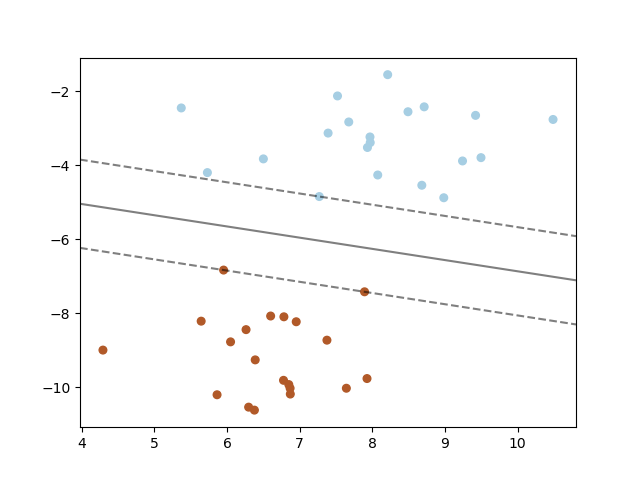
\includegraphics[width=0.5\textwidth]{images/svm_hiperplane}%
    \caption{Plano de separación de clases generado por una SVM}\label{fig:svm}
    \end{figure}

  \par SVR es una generalización de la SVM a problemas de regresión. Tecnicamente,
    se puede decir que es un algoritmo de aprendizaje supervisado. Éste
    requiere de un conjunto de datos de entrenamiento,
    $\mathcal{T} = (\vec{X}, \vec{Y})$, que cubre el dominio de interés acompañado
    de las soluciones en dicho dominio. El trabajo de la SVM es aproximar la función
    definida por el conjnuto de entrenamiento, $F(\vec{X}) = \vec{Y}$. En general,
    en las SVM, los vectores $\vec{X}$ son utilizados para definir el hiperplano que
    separa las distintas soluciones posibles. En problemas de regresión, estos
    vectores son utilizados para realizar una regresión lineal, los que estén
    más cerca del punto de prueba se los llama \textit{vectores de soporte}.

    Daremos una idea más detallada de los fundamentos matemáticos detrás de una
    SVR \cite{svr_tutorial}:

    Dados los vectores de entrenamiento $x_{i} \in \mathbb{R}^{p}$ con $i = 1, \dots ,n$
    y un vector $y \in \mathbb{R}$ el $\epsilon$-SVR resuelve el siguiente problema
    primario:

    \begin{align}
      \min\limits_{w, b, \zeta, \zeta^{*}} \frac{1}{2} w^{T} w + C \sum_{i = 1}^{n} \zeta_{i}
    \end{align}
    con las restricciones de:


    \begin{math}
      y_{i} - w^{T} \phi(x_{i}) - b \leq \epsilon + \zeta_{i}, \\
      w^{T} \phi(x_{i}) + b - y_{i} \leq \epsilon + \zeta^{*}_{i}, \\
            \zeta^{*}_{i}, \zeta_{i} \geq 0 \\
      para\ i\ =\ 1,\ \dots, n
    \end{math}

    Mientras que el problema dual a resolver es:

    \begin{align}
      \min\limits{\alpha, \alpha^{*}} \frac{1}{2} (\alpha - \alpha^{*})^{T}
      Q(\alpha - \alpha^{*}) + \epsilon e^{T} (\alpha + \alpha^{*}) -
      y^{T} (\alpha - \alpha^{*})
    \end{align}
    con las restricciones de:

    \begin{math}
      e^{T} (\alpha - \alpha^{*}) = 0, \\
      0 \geq \alpha, \alpha^{*} \leq C \\
      para\ i\ =\ 1, \dots, n
    \end{math}

  \par Donde $e$ es un vector para el cual todos sus componentes poseen el valor $1$, $C > 0$
    es la cota superior, $Q$ es una matriz semidefinida
    positiva\footnote{Una matriz, $M$, es semidefinida positiva si $x^{*}Mx \leq 0$
    $\forall x \in \mathbb{R}^{n}$} de tamaño $n \times n$,
    $Q_{ij} \equiv K(x_{i}, x_{j}) = \phi(x_{i}^{T})\phi(x_{j})$ es el núcleo
    (\textit{kernel}, en inglés). Aquí, los vectores de entrenamiento están siendo mapeados
    a un espacio de gran (probablemente infinita) dimensionalidad por la función
    $\phi$.
    Luego, la función de decisión es:
    \begin{align}
      \sum_{i = 1}^{n} (\alpha - \alpha^{*})K(x_{i}, x) + \rho
    \end{align}

\subsection{Perceptron Multicapa (MLP)}

  \par Un \textbf{Perceptron Multicapa} (MLP)\cite{mlp_intro1, mlp_intro2} es un tipo
    de red neuronal artificial (ANN) \textit{feedforward}.
    Éste es un algoritmo de aprendizaje supervisado que logra distinguir
    relaciones entre datos que no sean linealmente separables, aprende una función
    a partir de un conjunto de datos de entrenamiento y puede ser
    utilizada tanto para tareas de regresión como de clasificación haciendo uso, entre
    otras cosas, de una técnica llamada \textit{propagación hacia atrás}\cite{backpropagation}
    (\textit{backpropagation}, en inglés).
    El MLP consiste de al menos tres capas: una de entrada, una de salida y,
    como mínimo, una capa oculta\footnote{Una capa de neuronas artificiales que toman un conjunto
    de entradas ponderadas y producen una salida a través de una función de activación.};
    la vista gráfica de una arquitectura simple se puede observar en la
    Figura \ref{fig:mlp_ejemplo}.

  \par Una descripción matemática simplificada del algoritmo en cuestión es la
    que se menciona a continuación.
    Dados ejemplos de entrenamiento $(x_{1}, y_{1}), \dots, (x_{n}, y_{n})$
    donde $x_{i} \in \mathbb{R}^{n}$ y $y_{i} \in \{0,1\}$, un MLP de una capa oculta
    con una neurona aprende una función $f(x) = W_{2}g(W_{1}^{T} x + b_{1}) + b_{2}$
    donde $W_{1} \in \mathbb{R}^{m}$ y $W_{2}, b_{1}, b_{2} \in \mathbb{R}$ son
    parámetros del modelo. $W_{1}, W_{2}$ representan los pesos de la capa de entrada y la
    capa oculta, respectivamente. $b_{1}, b_{2}$ representan el sesgo agregado a
    la capa oculta y la capa de salida, respectivamente. La función
    $g(): \mathbb{R} \rightarrow \mathbb{R}$ es la función de activación, la cual
    es definida por defecto como la tangente hiperbólica. Está dada por,

    \begin{align}
      g(z) = \frac{e^{z} - e^{-z}}{e^{z} + e^{-z}}
    \end{align}

    En problemas de regresión, la salida del algoritmo es $f(x)$, por lo que la
    función de activación de salida es simplemente la función identidad. En estos
    problemas, MLP también utiliza como función de pérdida la correspondiente
    al \textit{Error Cuadrático}:
    \begin{align}
      Loss(\hat{y}, y, W) = \frac{1}{2} \norm{\hat{y} - y}^{2}_{2} + \frac{\alpha}{2} \norm{W}^{2}_{2}
    \end{align}



  \par Comenzando desde pesos con valores aleatorios, el MLP minimiza la función de
    pérdida actualizando repetidamente dichos pesos. Luego de calcular la pérdida,
    se propaga desde la capa de salida a todas las anteriores (\textit{backpropagation}),
    proporcionando un valor de peso a cada parámetros para disminuir la pérdida.
    Para ello, se utiliza \textit{descenso por gradiente}, en el cual el
    gradiente $\nabla Loss_{W}$ de la pérdida con respecto a los pesos es
    calculada y deducida de W.
    Más formalmente, es expresado como:
    \begin{align}
      W^{i + 1} = W^{i} - \epsilon \nabla Loss^{i}_{W}
    \end{align}
    donde $i$ es el paso de iteración, y $\epsilon > 0$ es la taza de aprendizaje.

    En general el algoritmo termina cuando se alcanza cierto número definido por el
    usuario de iteraciones o se cruza un humbral para la pérdida.

    \begin{figure}
    \centering%
    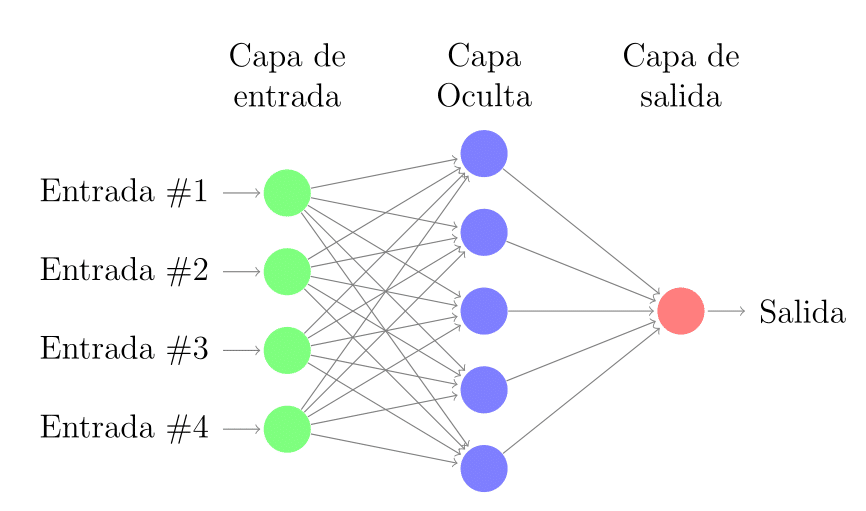
\includegraphics[width=0.7\textwidth]{images/ejemplo_mlp}%
    \caption{Arquitectura de una MLP de cuatro variables de entrada, una capa
            oculta de cinco neuronas y un sólo valor de salida}\label{fig:mlp_ejemplo}
    \end{figure}


\end{document}
